\documentclass[UTF8,a4paper,11pt]{ctexart}

\usepackage[margin=2.2cm]{geometry}
\usepackage{graphicx}
\usepackage{booktabs}
\usepackage{array}
\usepackage{float}
\usepackage{xcolor}
\usepackage{hyperref}
\usepackage{enumitem}
\usepackage{amsmath}
\usepackage{amssymb}
\usepackage{caption}

\hypersetup{
  colorlinks=true,
  linkcolor=blue!50!black,
  citecolor=blue!50!black,
  urlcolor=blue!50!black
}

\setlist[itemize]{leftmargin=1.8em}
\setlist[enumerate]{leftmargin=1.8em}
\captionsetup{font=small,labelfont=bf}

\title{\heiti 无病灶标注条件下腹膜后肿瘤CT二分类筛查模型的初步研究}
\author{J. Ho \quad Codex 协作整理}
\date{2026年7月}

\begin{document}

\maketitle

\begin{abstract}
目的：在缺乏医生逐层肿瘤ROI标注的现实条件下，构建一个可复现、低成本的腹膜后肿瘤CT二分类筛查模型，用于区分“良性神经源性肿瘤”和“非良性/需处理病变”。方法：本研究整理246例腹膜后肿瘤增强CT病例，其中良性神经源性肿瘤55例，非良性/需处理病变191例，后者包括肉瘤类、淋巴瘤、嗜铬细胞瘤/副神经节瘤和胃肠道间质瘤。模型不使用分割掩膜或肿瘤中心点，而是将每例CT表示为96张轴位切片；每张切片经三种CT窗动态转换为三通道图像，并由ImageNet预训练ResNet18提取切片特征。随后使用基于mean/max pooling的2.5D弱监督多实例学习框架进行病例级分类，并融合年龄、性别等表格特征。评价采用患者级五折交叉验证，重点关注非良性/需处理病变被误判为良性的假阴性风险。结果：主模型在合并五折测试集上取得Accuracy 0.821、Balanced Accuracy 0.691、Macro-F1 0.711、Sensitivity 0.927、Specificity 0.455、AUROC 0.670、Average Precision 0.848。混淆矩阵显示191例非良性/需处理病例中177例被正确识别，假阴性14例；55例良性神经源性肿瘤中25例被正确识别，30例被判为非良性/需处理。结论：在无ROI标注条件下，2.5D弱监督MIL结合年龄/性别特征可以形成一个可运行的腹膜后肿瘤筛查式二分类基线。当前模型更适合作为“尽量不漏掉需处理病变”的初步筛查工具，而不能作为临床诊断模型。
\end{abstract}

\noindent\textbf{关键词：} 腹膜后肿瘤；CT；弱监督学习；多实例学习；ResNet18；二分类筛查

\section{引言}

腹膜后肿瘤病理类型复杂，影像表现具有一定重叠性。在正式临床诊断中，病理学结论仍是金标准；影像模型若要达到临床可用水平，通常需要更大的样本、多中心外部验证，以及由医生标注的肿瘤区域。然而在当前数据条件下，逐层分割ROI的成本过高，且已有数据主要是病例级诊断标签。因此，本研究没有复刻基于病灶分割的分类路线，而是将问题重新定义为一个更务实的弱监督筛查任务。

本研究的主任务不是严格病理学意义上的“良恶性分类”，而是：

\begin{quote}
良性神经源性肿瘤 vs 非良性/需处理腹膜后病变。
\end{quote}

这一设定的临床含义更接近“哪些病例不能简单视作普通良性神经源性肿瘤”。其中嗜铬细胞瘤/副神经节瘤（PPGL）并不被简单称为恶性，但其临床处理方式、术前评估和风险管理均不同于普通良性神经源性肿瘤，因此被归入“非良性/需处理病变”。

\section{材料与方法}

\subsection{数据集与标签定义}

本研究共纳入246例可用增强CT病例。标签由既有病例表格整理得到，最终固定为二分类任务。类别构成见表\ref{tab:dataset}。

\begin{table}[H]
  \centering
  \caption{二分类标签构成}
  \label{tab:dataset}
  \begin{tabular}{llr}
    \toprule
    二分类标签 & 纳入原始类别 & 例数 \\
    \midrule
    良性神经源性肿瘤 & 良性神经源性肿瘤 & 55 \\
    非良性/需处理病变 & 肉瘤类 & 103 \\
     & 淋巴瘤 & 44 \\
     & PPGL & 30 \\
     & 胃肠道间质瘤 & 14 \\
    \midrule
    合计 &  & 246 \\
    \bottomrule
  \end{tabular}
\end{table}

所有训练、验证和测试划分均按患者级别进行，避免同一患者不同序列或派生样本跨集合造成数据泄漏。实验采用五折交叉验证，并将每折测试结果合并后计算总体指标。

\subsection{影像预处理}

每例CT以NIfTI格式读取。模型输入不依赖人工肿瘤框、分割掩膜或点击点，而是直接使用整套CT。预处理流程如下：

\begin{enumerate}
  \item 沿轴位方向从每例CT中采样96张切片。
  \item 每张切片resize至$224 \times 224$。
  \item 将HU值转换为三通道CT窗图像：
  \begin{itemize}
    \item 软组织窗：$[-160, 240]$；
    \item 脂肪敏感窗：$[-200, 100]$；
    \item 宽腹部窗：$[-200, 400]$。
  \end{itemize}
  \item 每个窗内线性归一化到$[0,1]$，随后使用ImageNet均值和标准差进行标准化，以适配预训练ResNet18。
\end{enumerate}

三窗设置的动机是尽量同时保留软组织密度、脂肪成分和较宽范围腹部结构信息。对于脂肪肉瘤等病变，脂肪成分具有潜在诊断价值；对于淋巴瘤、PPGL和其他实体肿瘤，软组织窗和宽窗则可能提供更稳定的密度与解剖背景。

\subsection{模型结构}

模型采用2.5D弱监督多实例学习（multiple instance learning, MIL）框架。每例CT被视为一个bag，96张轴位切片为instances。整体结构如图\ref{fig:model_metrics}所示，并可形式化为：

\[
x = \{x_1, x_2, \ldots, x_{96}\}, \quad f_i = \mathrm{ResNet18}(x_i), \quad f_i \in \mathbb{R}^{512}
\]

其中ResNet18使用ImageNet预训练权重，并作为切片级特征提取器。每例CT的影像特征由切片特征的mean pooling和max pooling组合得到：

\[
h_{\mathrm{img}} = [\mathrm{mean}(f_1,\ldots,f_{96});\ \mathrm{max}(f_1,\ldots,f_{96})]
\]

表格特征包括年龄与性别。主模型使用影像分支和表格分支的晚期融合：影像分支输出病例级非良性/需处理概率，表格分支输出基于年龄/性别的概率，最终以等权方式得到融合预测。该设计有三个优点：一是代码较简洁；二是可以直接检查影像分支和表格分支各自贡献；三是在小样本条件下比端到端训练大模型更稳定。

\begin{figure}[H]
  \centering
  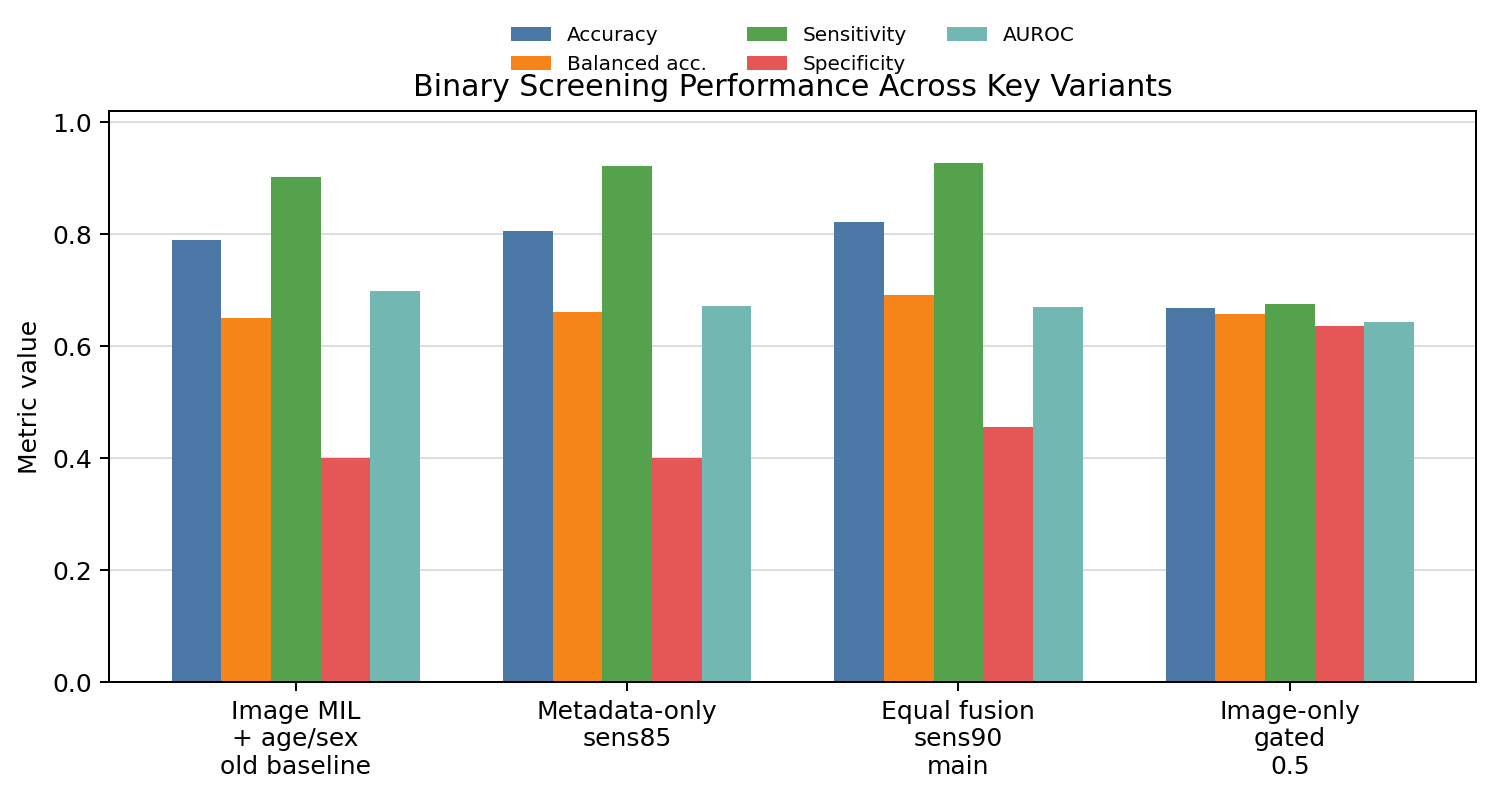
\includegraphics[width=0.95\linewidth]{figures/model_comparison_metrics.png}
  \caption{关键模型变体在合并五折测试集上的表现。主模型为影像MIL与年龄/性别表格特征等权融合，并采用验证集选择的高敏感度阈值。}
  \label{fig:model_metrics}
\end{figure}

\subsection{训练与评价}

本研究将“非良性/需处理病变”作为筛查任务中的阳性类，因此评价时尤其关注阳性类敏感度，即非良性/需处理病例不被漏诊的比例。主报告指标包括Accuracy、Balanced Accuracy、Macro-F1、Sensitivity、Specificity、AUROC和Average Precision。

由于类别不平衡，Accuracy不能单独反映模型质量。对于本任务而言，假阴性（非良性/需处理病变被判定为良性神经源性肿瘤）比假阳性更加值得警惕。因此，主模型采用验证集选择的高敏感度工作点，目标是提高阳性类检出率，同时保留一定良性识别能力。

\section{结果}

\subsection{总体性能}

表\ref{tab:main_results}总结了主要模型及对照实验结果。当前主模型为“ResNet18 2.5D MIL + 年龄/性别等权融合 + 高敏感度阈值”。其合并五折测试结果为Accuracy 0.821、Balanced Accuracy 0.691、Macro-F1 0.711、Sensitivity 0.927、Specificity 0.455、AUROC 0.670、Average Precision 0.848。

\begin{table}[H]
  \centering
  \caption{主要模型与对照结果}
  \label{tab:main_results}
  \resizebox{\linewidth}{!}{%
  \begin{tabular}{lccccccc}
    \toprule
    模型 & Acc & BAcc & Macro-F1 & Sens & Spec & AUROC & AP \\
    \midrule
    Image MIL + 年龄/性别，旧基线 & 0.789 & 0.650 & 0.664 & 0.901 & 0.400 & 0.698 & 0.863 \\
    年龄/性别 only & 0.805 & 0.661 & 0.679 & 0.921 & 0.400 & 0.671 & 0.869 \\
    \textbf{Image MIL + 年龄/性别等权融合，主模型} & \textbf{0.821} & \textbf{0.691} & \textbf{0.711} & \textbf{0.927} & \textbf{0.455} & 0.670 & 0.848 \\
    Image-only gated MIL & 0.667 & 0.656 & 0.610 & 0.675 & 0.636 & 0.643 & 0.850 \\
    \bottomrule
  \end{tabular}
  }
\end{table}

混淆矩阵见图\ref{fig:cm}。在191例非良性/需处理病变中，177例被正确判为阳性，14例被误判为良性神经源性肿瘤；在55例良性神经源性肿瘤中，25例被正确判为阴性，30例被判为阳性。

\begin{figure}[H]
  \centering
  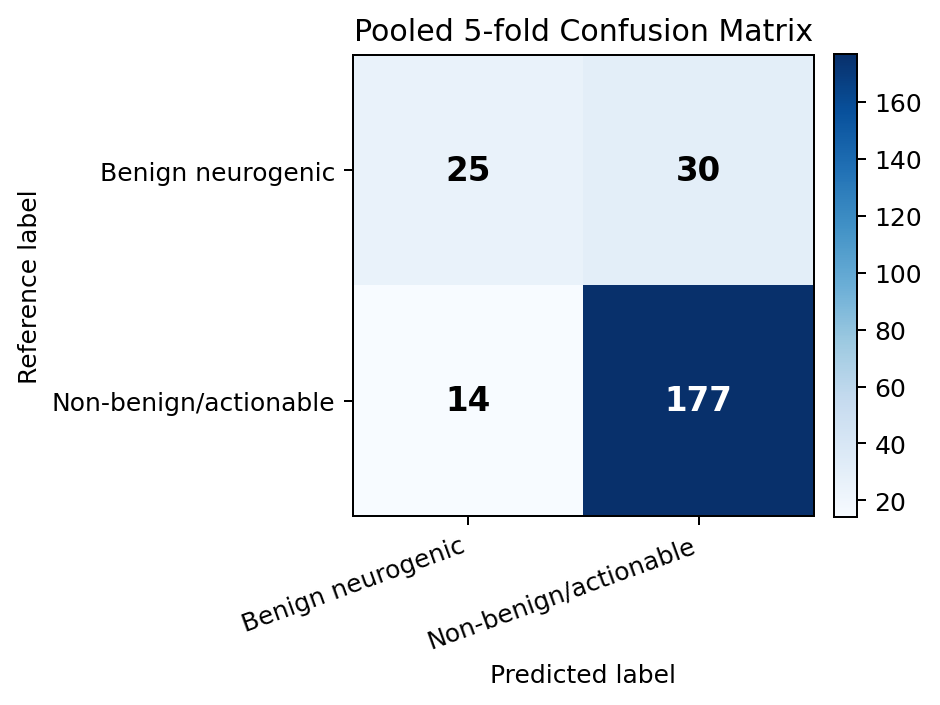
\includegraphics[width=0.72\linewidth]{figures/main_confusion_matrix.png}
  \caption{主模型合并五折测试集混淆矩阵。行表示真实标签，列表示预测标签。}
  \label{fig:cm}
\end{figure}

\subsection{按原始病理分组的召回表现}

进一步按原始病理分组统计召回率，结果见表\ref{tab:subtype}. 主模型对肉瘤类、PPGL、淋巴瘤和胃肠道间质瘤均保持较高召回率，说明模型在筛查“需处理病变”时有一定积极信号。但良性神经源性肿瘤的特异度只有0.455，意味着仍有较多良性病例被模型判为需处理。

\begin{table}[H]
  \centering
  \caption{主模型按原始类别统计的召回表现}
  \label{tab:subtype}
  \begin{tabular}{lrr}
    \toprule
    原始类别 & 例数 & 召回率 \\
    \midrule
    肉瘤类 & 103 & 0.932 \\
    PPGL & 30 & 0.933 \\
    淋巴瘤 & 44 & 0.932 \\
    胃肠道间质瘤 & 14 & 0.857 \\
    良性神经源性肿瘤 & 55 & 0.455 \\
    \bottomrule
  \end{tabular}
\end{table}

\subsection{预处理与增强消融}

为了验证更复杂预处理是否能提升结果，本研究额外尝试了body crop、多视角数据增强、不同切片采样策略和不同CT窗设置。结果如图\ref{fig:ablation}和表\ref{tab:ablation}所示。

\begin{figure}[H]
  \centering
  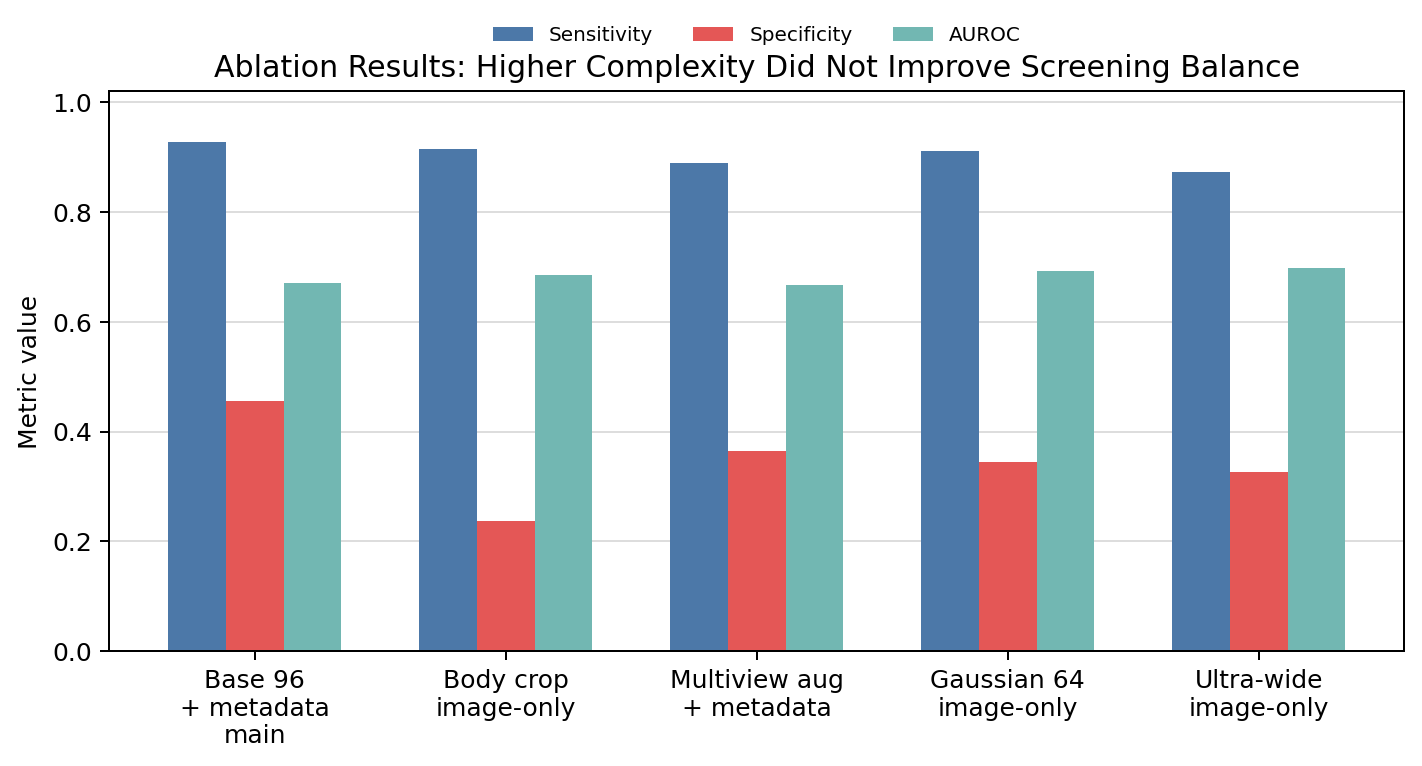
\includegraphics[width=0.95\linewidth]{figures/ablation_summary.png}
  \caption{预处理与增强消融实验。更复杂的body crop、多视角增强或切片/窗宽调整并未稳定优于当前主模型。}
  \label{fig:ablation}
\end{figure}

\begin{table}[H]
  \centering
  \caption{预处理和增强实验摘要}
  \label{tab:ablation}
  \resizebox{\linewidth}{!}{%
  \begin{tabular}{lcccccc}
    \toprule
    实验 & Acc & BAcc & Macro-F1 & Sens & Spec & AUROC \\
    \midrule
    主模型：96切片 + 三窗 + 年龄/性别融合 & 0.821 & 0.691 & 0.711 & 0.927 & 0.455 & 0.670 \\
    Body crop image-only & 0.764 & 0.576 & 0.584 & 0.916 & 0.236 & 0.686 \\
    多视角增强 + 年龄/性别融合 & 0.772 & 0.627 & -- & 0.890 & 0.364 & 0.667 \\
    高斯采样64切片 image-only & 0.785 & 0.628 & -- & 0.911 & 0.345 & 0.693 \\
    超宽窗96切片 image-only & 0.752 & 0.601 & -- & 0.874 & 0.327 & 0.699 \\
    \bottomrule
  \end{tabular}
  }
\end{table}

这些结果提示：当前主要瓶颈不一定是切片数量或窗宽窗位设置本身，而可能来自病例量、标签噪声、影像表型重叠以及缺乏病灶定位。Body crop虽然可以去掉部分空气背景，但实际裁剪区域仍接近全腹部，并没有真正定位肿瘤。多视角增强也未改善筛查工作点，反而使假阴性略有增加。因此，在当前阶段保留更简洁的96切片三窗输入更合理。

\section{讨论}

\subsection{为什么二分类比多分类更适合当前数据}

早期实验尝试过五分类、七分类和3D模型，但在当前样本量下，各少数类的稳定评估较困难，且模型容易过拟合。相比之下，“良性神经源性肿瘤 vs 非良性/需处理病变”的二分类任务更贴近当前数据规模，也更符合临床筛查逻辑：我们最担心的不是把良性病例多判为需处理，而是把肉瘤、淋巴瘤、PPGL或GIST误判为普通良性神经源性肿瘤。

因此，主模型优先选择高敏感度阈值。结果中14例非良性/需处理病变被误判为良性，这是目前最需要继续分析的错误类型；而30例良性神经源性肿瘤被判为需处理，虽然会降低特异度，但在筛查场景下相对可接受。

\subsection{年龄和性别特征的意义}

年龄、性别等表格特征在本任务中提供了明显增益。需要强调的是，这既可能反映真实流行病学差异，也可能反映当前数据集中的采样偏倚。因此，本研究没有将表格特征解释为病理机制，而是将其作为提高筛查性能的辅助变量。未来若进行外部验证，应单独报告影像only模型、表格only模型和融合模型，避免把数据集偏倚误认为影像模型能力。

\subsection{为什么没有采用分割或TotalSegmentator}

本研究没有使用肿瘤分割，原因有二。第一，当前数据没有医生逐层ROI标注，硬做分割式分类会显著增加人工成本。第二，探索性实验显示，通用解剖分割或粗略body crop只能提供身体范围或大腹部范围，不能可靠定位腹膜后肿瘤本身。因此，这类方法目前不能替代病灶ROI。若后续有人工粗框或肿瘤中心点，则更值得尝试的是“粗定位+MIL”而不是全自动通用器官分割。

\subsection{局限性}

本研究仍有明显局限：

\begin{itemize}
  \item 数据量仍偏小，且缺乏独立外部测试集；
  \item 当前结果来自内部五折交叉验证，不应等同于真实临床泛化性能；
  \item 没有病灶分割、粗框或医生ROI，模型可能学习到与肿瘤无关的背景差异；
  \item 年龄和性别特征可能带来数据集偏倚；
  \item 良性神经源性肿瘤特异度仍较低，模型会将较多良性病例判为需处理；
  \item PPGL被归入“非良性/需处理”是临床任务定义，不是将其简单等同于恶性肿瘤。
\end{itemize}

\section{结论}

本研究构建了一个无ROI标注条件下的腹膜后肿瘤CT二分类筛查基线。基于96张轴位切片、三窗输入、ResNet18切片特征和2.5D MIL聚合，并融合年龄/性别信息后，模型在246例内部五折交叉验证中实现了较高的非良性/需处理病变敏感度。当前结果说明该路线具备作为初步筛查实验的可行性，但尚不足以支持临床诊断应用。后续工作应优先补充外部验证集、进行病例级错误分析，并在可承受人工成本的前提下探索粗框或中心点辅助定位。

\section*{代码与数据说明}

项目代码、标签说明和报告文件保存在私有Git仓库中。原始NIfTI、缓存tensor、ResNet特征tensor和模型权重不纳入Git版本控制，以避免隐私和仓库体积问题。当前主线训练入口为二分类影像-表格融合模型；旧的五分类、3D、分割和41例小试验分支已从当前工作树移除，仅保留在Git历史中可追溯。

\begin{thebibliography}{9}
  \bibitem{resnet}
  He K, Zhang X, Ren S, Sun J. Deep Residual Learning for Image Recognition. Proceedings of the IEEE Conference on Computer Vision and Pattern Recognition; 2016.

  \bibitem{mil}
  Ilse M, Tomczak J, Welling M. Attention-based Deep Multiple Instance Learning. International Conference on Machine Learning; 2018.

  \bibitem{imagenet}
  Deng J, Dong W, Socher R, Li L-J, Li K, Fei-Fei L. ImageNet: A Large-Scale Hierarchical Image Database. IEEE Conference on Computer Vision and Pattern Recognition; 2009.
\end{thebibliography}

\end{document}
